
%% * Introduce the RL setup
%% * Define formally the RL setup using MDPs
%% * Give some examples of MDPs
%% * Give some hints about POMDPs

\subsection{The problem} \title{Defining the RL framework} \author{} \date{}
\begin{frame}[plain,c]
    \titlepage
\end{frame}

\begin{frame}
    \frametitle{Agent-environment interaction}
    \begin{figure}
        \centering
        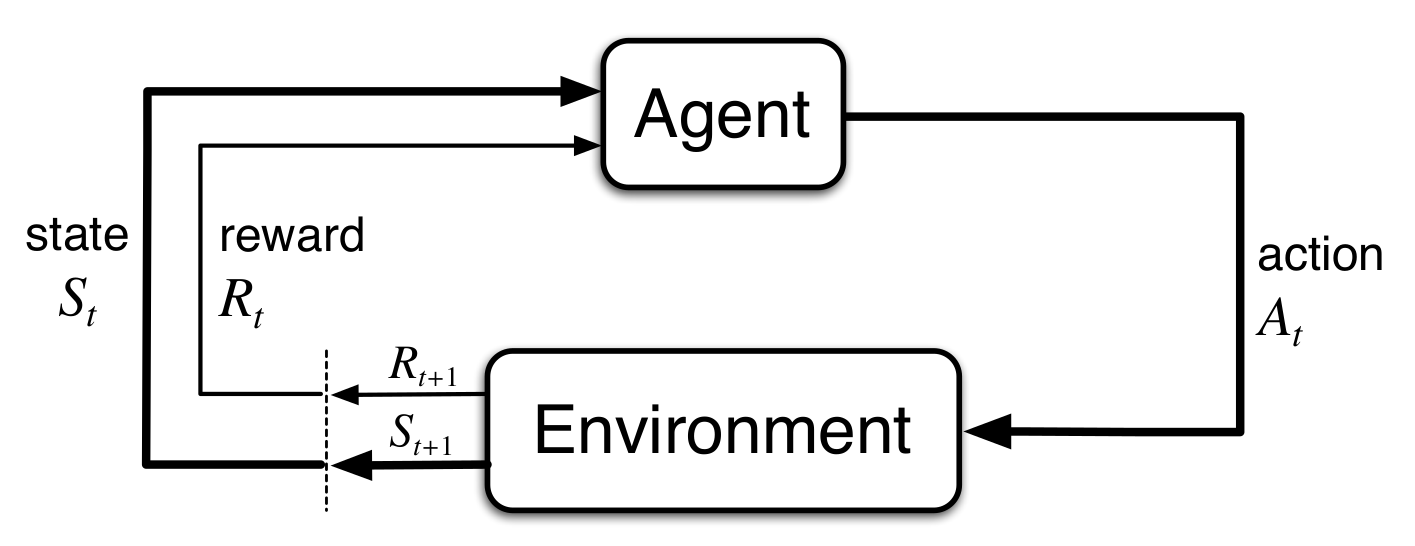
\includegraphics[width=0.6\textwidth]{./imgs/img_rl_loop.png}
        \caption{RL interaction loop \cite{RLbook}}
    \end{figure}

    \pause

    \begin{itemize}
        \item State $s_{t}$: configuration of the world. \pause
        \item Action $a_{t}$: available ways to act in the world. \pause
        \item Environment: dynamics of the world the agent lives in. \pause
        \item Reward $r_{t+1}$: reward given by the world for our transition. \pause
        \item Next state $s_{t+1}$: next state the agent lands in the world.
    \end{itemize}
\end{frame}

\begin{frame}
    \frametitle{Example: Locomotion}
    \begin{figure}
        \centering
        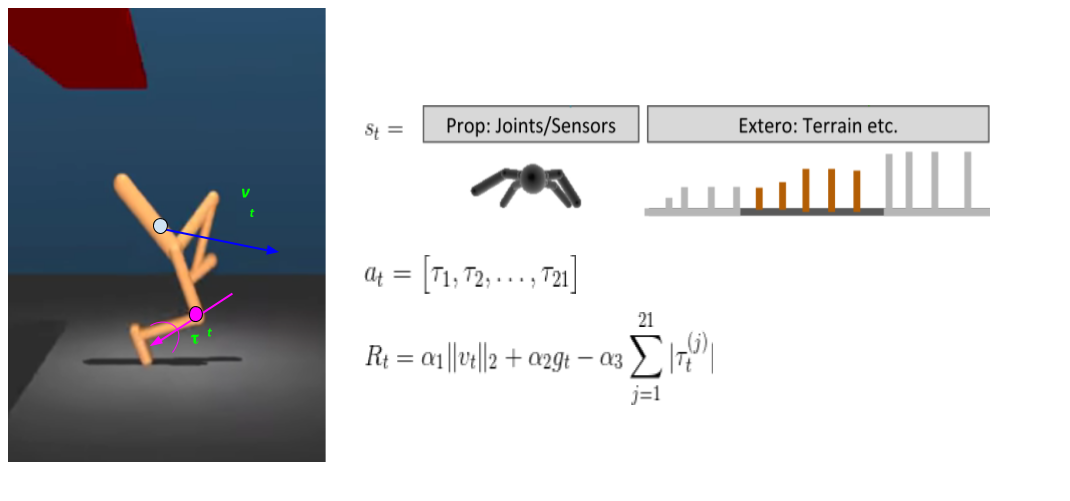
\includegraphics[width=\textwidth]{./imgs/img_rl_mdp_locomotion.png}
    \end{figure}
\end{frame}

\begin{frame}
    \frametitle{Example: Atari games}
    \begin{figure}
        \centering
        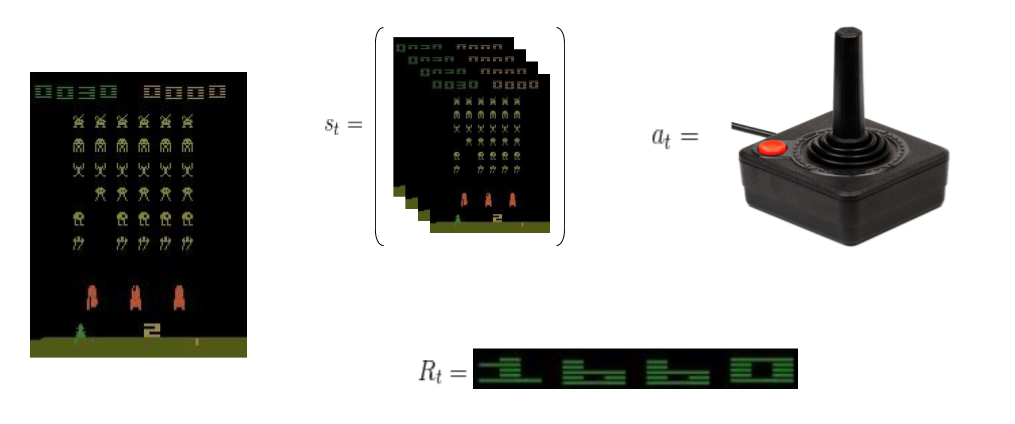
\includegraphics[width=\textwidth]{./imgs/img_rl_mdp_atari.png}
    \end{figure}
\end{frame}

\begin{frame}
    \frametitle{Mathematical Formulation: Markov Decision Processes}
    \begin{block}{Markov Decision Process}
        A Markov Decision Process is a mathematical framework for sequential
        decision making under uncertainty, defined by the tuple $(S,A,P,R)$ :
        \begin{itemize}
            \item $S=\left \{ s \right \}$: State space.
            \item $A=\left \{ a \right \}$: Action space.
            \item $P=p(s'|s,a)$: Transition model.
            \item $R(s)$ or $R(s,a)$ or $R(s,a,s')$: Reward function.
        \end{itemize}
    \end{block}

    \pause

    \begin{figure}
        \centering
        \begin{subfigure}{0.18\textwidth}
            \centering
            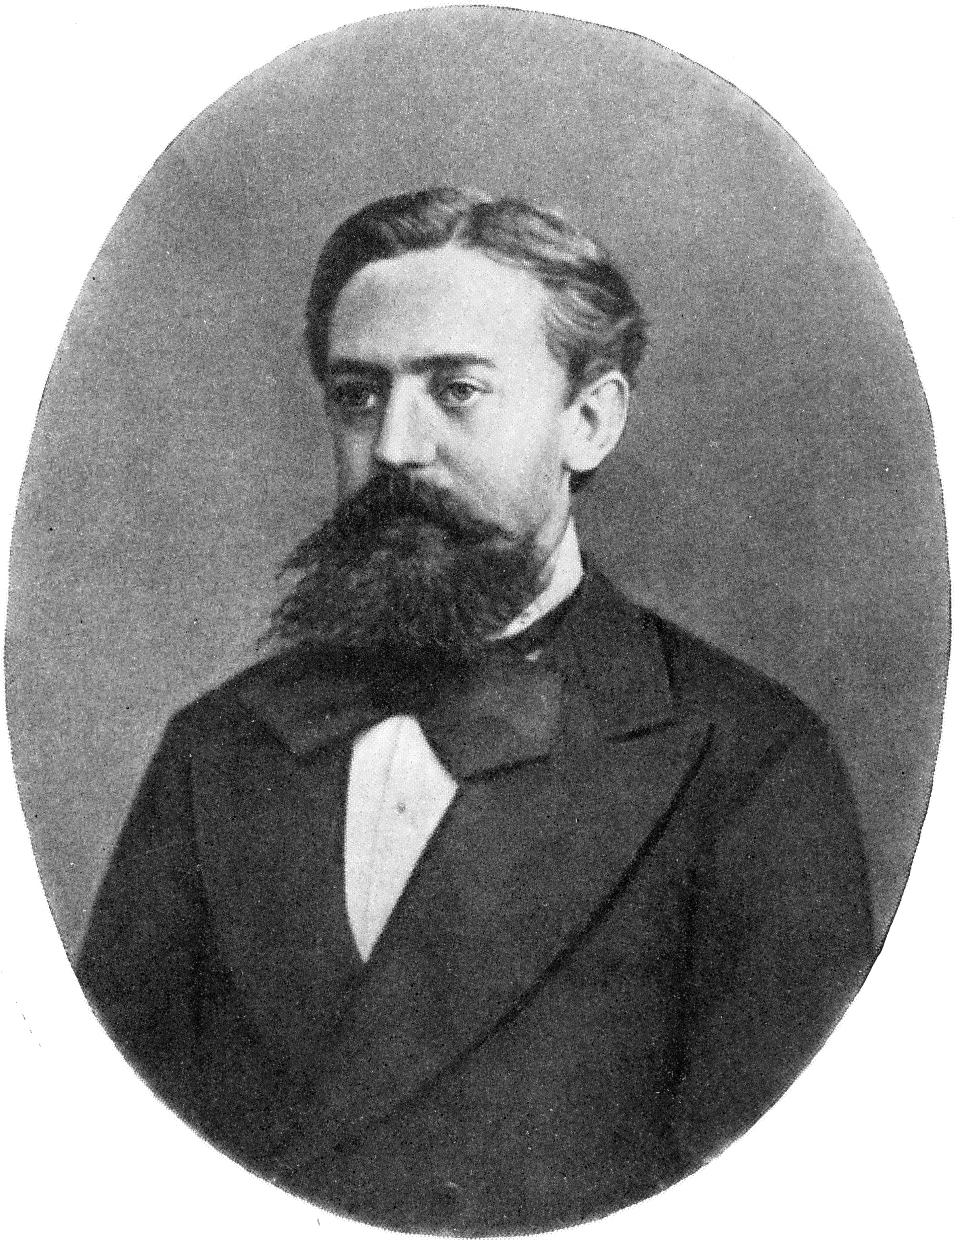
\includegraphics[width=0.9\textwidth]{./imgs/img_rl_mdp_andrey_markov.png}
            \caption{Andrey Markov}
        \end{subfigure}
        \hspace{0.1\textwidth}
        \begin{subfigure}{0.4\textwidth}
            \centering
            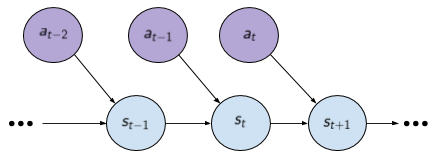
\includegraphics[width=0.9\textwidth]{./imgs/img_rl_mdp_graphical_model.png}
            \caption{Graphical model of an MDP}
        \end{subfigure}
    \end{figure}
\end{frame}

\begin{frame}
    \frametitle{A simple recycling robot MDP}
    \begin{figure}
        \centering
        \begin{subfigure}{0.45\textwidth}
            \centering
            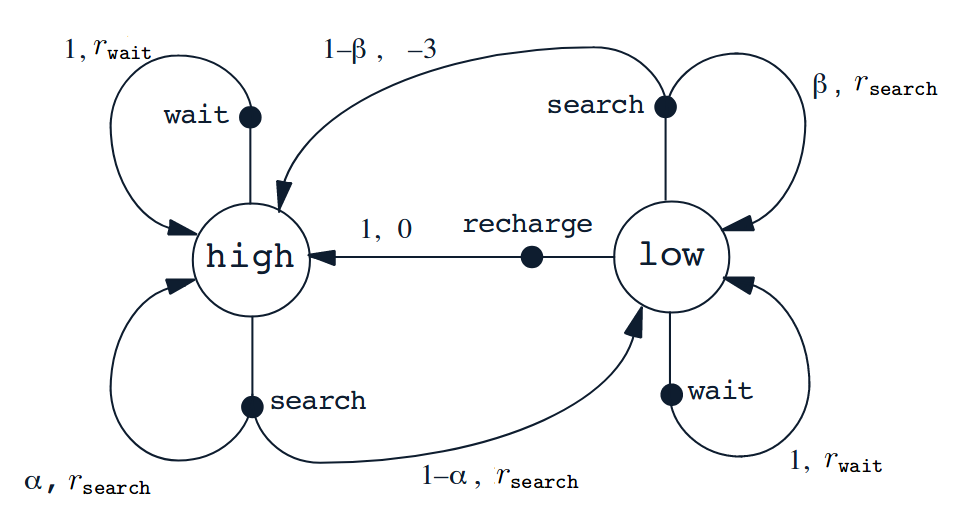
\includegraphics[width=0.9\textwidth]{./imgs/img_rl_mdp_robot_cleaner_1.png}
            \caption{MDP of a recycling robot}
        \end{subfigure}
        \pause
        \begin{subfigure}{0.45\textwidth}
            \centering
            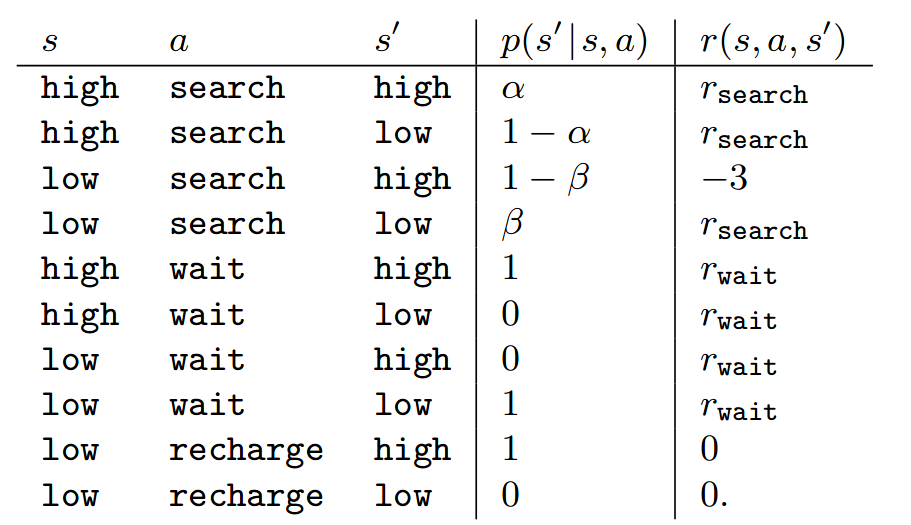
\includegraphics[width=0.9\textwidth]{./imgs/img_rl_mdp_robot_cleaner_2.png}
            \caption{Transition dynamics of the recycling robot MDP}
        \end{subfigure}
    \end{figure}
\end{frame}

\begin{frame}
    \frametitle{Another simple example}
    \begin{figure}
        \centering
        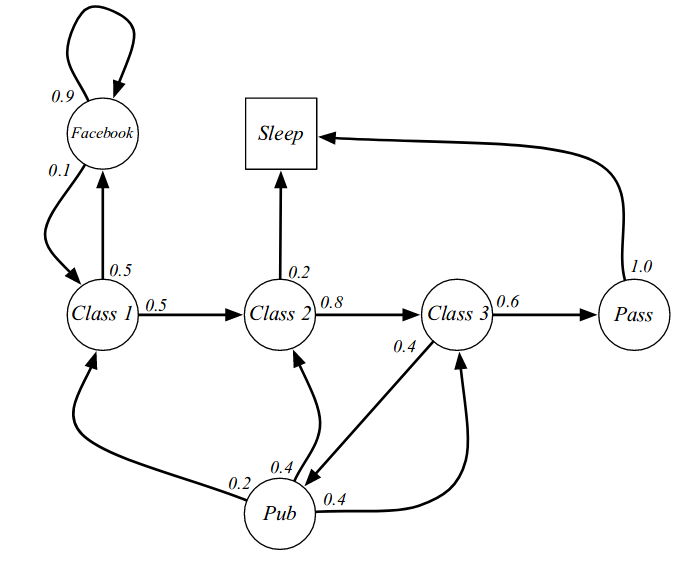
\includegraphics[width=0.5\textwidth]{./imgs/img_rl_mdp_student_example.png}
        \caption{Another example of an MDP}
    \end{figure}
\end{frame}

\begin{frame}
    \frametitle{Does the Markov assumption hold?}
    \begin{itemize}
        \item In general, we don't always have access to the full state
              of the environment $s_{t}$.
        \item Instead, we usually just have access to some observation
              $o_{t}$ (generated from $s_{t}$) which gives less information.
        \item Because of this, we might not be able to recover the full state
              of the environment from the observations we have.
    \end{itemize}

    \pause

    \begin{figure}
        \centering
        \begin{subfigure}{0.3\textwidth}
            \centering
            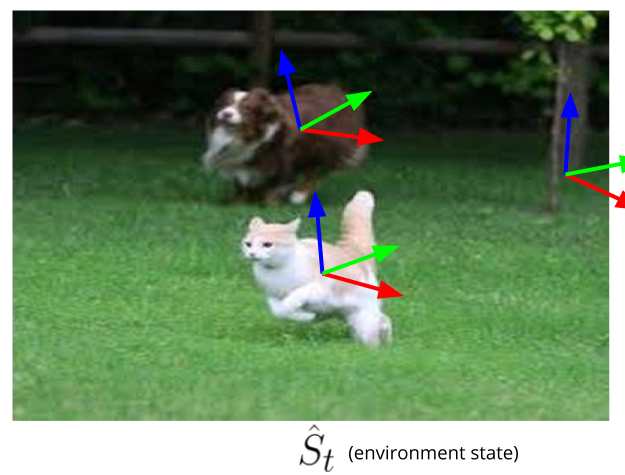
\includegraphics[width=0.9\textwidth]{./imgs/img_rl_pomdp_example_2.png}
        \end{subfigure}
        \begin{subfigure}{0.3\textwidth}
            \centering
            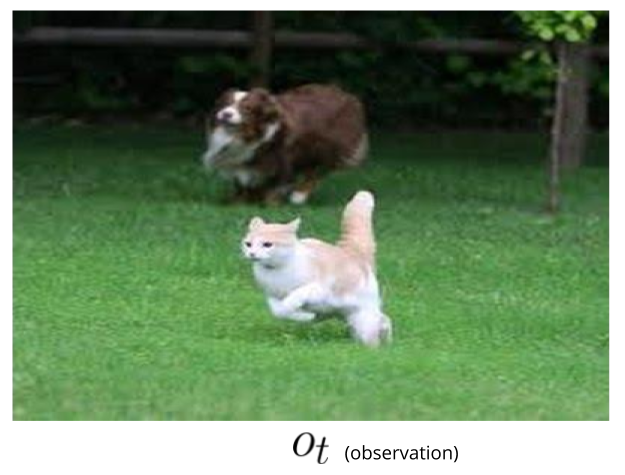
\includegraphics[width=0.9\textwidth]{./imgs/img_rl_pomdp_example_1.png}
        \end{subfigure}
        \begin{subfigure}{0.3\textwidth}
            \centering
            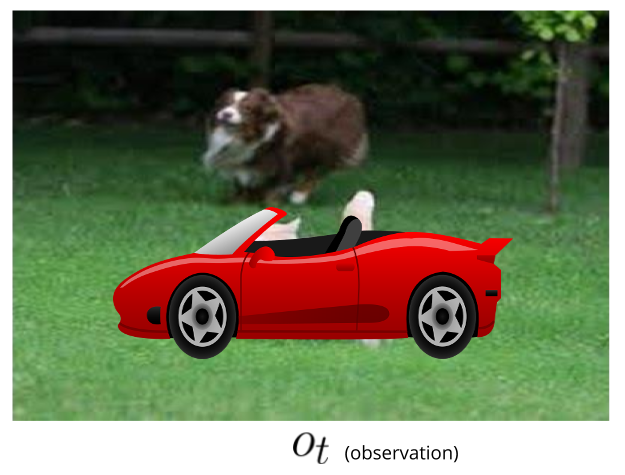
\includegraphics[width=0.9\textwidth]{./imgs/img_rl_pomdp_example_3.png}
        \end{subfigure}
    \end{figure}
\end{frame}

\begin{frame}
    \frametitle{Partially Observable MDPs (POMDPs)}
    \begin{block}{Partially Observable Markov Decision Processes (POMDP)}
        A POMDP is an MDP with hidden states defined by the following:
        \begin{itemize}
            \item $S=\left \{ s \right \}$: State space.
            \item $A=\left \{ a \right \}$: Action space.
            \item $\Omega=\left \{ o \right \}$: Observation space.
            \item $P=p(s'|s,a)$: Transition model.
            \item $R(s)$ or $R(s,a)$ or $R(s,a,s')$: Reward function.
            \item $Z=p(o|s)$: Observation model
        \end{itemize}
    \end{block}

    \pause

    \begin{figure}
        \centering
        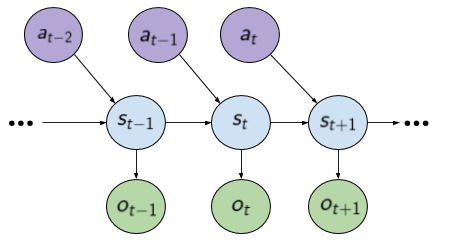
\includegraphics[width=0.4\textwidth]{./imgs/img_rl_pomdp_graphical_model.png}
    \end{figure}
\end{frame}

\begin{frame}
    \frametitle{What's the objective of the agent?}
    \begin{block}{Try 1: Maximize reward?}
        \begin{itemize}
            \item $\max r_{t+1}$ ???
            \pause
            \item Not really, as doing only good things \textbf{now} does
                  not guarantee that we do well in the long-run.
        \end{itemize}
    \end{block}
    \pause
    \begin{block}{Try 2: Maximize sum of rewards?}
        \begin{itemize}
            \item $\max \sum_{t=1}^{T} r_{t}$
            \pause
            \item Almost. Recall that the environment might be stochastic.
        \end{itemize}
    \end{block}
    \pause
    \begin{block}{RL objective}
        \begin{equation*}
            \max \mathbb{E} \left \{ \sum_{t=1}^{T} r_{t} \right \}
        \end{equation*}
    \end{block}
\end{frame}